\chapter{Introduction}
\label{ch:Introduction}
% 1) Few words on the need of optical communications

% 2) Need of narrow linewidth lasers in coherent communication systems

% 3) Need of directly modulated lasers in fiber-to-the-home (FTTH) or passive optical networks (PON)

% 4) Scope of this work: explore the possibility of using feedback in polymer-based tunable lasers as a to reduce linewidth for coherent communication systems, and increase of bandwidth (and reduction of chirp) for e.g. FTTH and PON, 



% \section{Tunable Lasers in Integrated Optics}
% The huge possibilities of digital interfaces have an impact on the optical line interfaces of the edge switches and the data-center gateways. Current 100G implementations based on dual-polarization quadrature phase-shift keying are becoming obsolete and we can expect the next migration from 100G to 400G and even further on to 1T based on higher quadrature amplitude modulation (QAM) formats. The aim of the research is to integrate a highly-functional coherent receiver chip, which includes an optical 90° hybrid as the frontend to convert the phase modulated signal into amplitude modulated signal detectable by photodiodes (PDs) [4-6], variable optical attenuators (VOAs) and a wavelength-tunable local oscillator (LO). Everything is done on PolyBoard (polymer-based hybrid platform). This technology allows inserting thin-film elements (TFEs) as polarizations rotators (PR) and polarization beam splitters (PBS). Lasing can be achieved by coupling an InP gain chip (GC) to a polymer Bragg grating. As 90° hybrids 2x4 MMI are used, as VOAs, thermally tunable 1x1 MMIs. This receiver component aims to serve as a potential candidate for 1 Tb/s transceivers for data-centers.

Increasing demand of high speed data transmission is affecting people's daily life and more advanced optcial communication technology is needed to full this request, integrated tunable semiconductor laser is one of the important technologies.

% using narrow linewidth lasers in coherent communication systems and directly modulated lasers in Fiber-To-The-Home (FTTH) or Passive Optical Networks (PON).



% %%%%%%%%%%%%%%%%%%%%%%%%% Cohehent %%%%%%%%%%%%%%%%%%%%%%
The use of coherent communication in optical network systems is spreading rapidly to increase the transmission capacity \cite{ishii2017narrow}, it is considered as a promising key technology to increase the spectral efficiency of optical transmission and to overcome the future capacity limitations of the currently installed fibre infrastructure \cite{seimetz2008laser}. Laser used in such systems requires narrow spectral linewidth because of the usage of the higher-oder multi-level modulation format, such as 64QAM or beyond \cite{seimetz2008laser}. Single-frequency laser diodes such as Didtributed Bragg Refelctor (DBR) laser appears to be a good candidate for achieving narrow linewidth. Recently, linewidths of 350 kHz have been achieved \cite{de2016hybrid}, however, it is still limited by the short photon lifetime because of the relative short laser cavity. 
Concept of hybrid tunable lasers \cite{fan2017spectral}, which consists of an active section coupled to a passive waveguide section comprising tunable filters and reflectors, permits a narrower linewidth due to increased photon lifetime that is associted with an extended cavity length \cite{henry1982theory}.

% The spectral linewidth of the laser affects the performance of these systems.
% Coherent optical communication systems are gaining rapid importance because they allow to increase the speed (data rate) of transmission, by making use of the phase-predicatability of lasers with narrow spectral linewidth.

% %%%%%%%%%%%%%% Direct modulation %%%%%%%%%%%%%%%%%%%%%%%%%%
Besides, the directly modulated laser is a simple and reliable source for high speed optical communication. It is especially useful in short to medium distance applications (e.g. local area networks \cite{zhang2012next} and optical interconnects \cite{taubenblatt2012optical}) where the excess pulse dispersion due to laser chirp is not a critical issue \cite{soriano2013complex}. It represents a relevant element to fulfill the continuously increasing need for low-cost optical communications systems with high bit-rate such as Fiber-To-The-Home (FTTH) \cite{cartaxo2011perspective, khanaa2013performance} and Passive Optical Network (PON) \cite{urata2012high, kani2010enabling} technology. In order to achieve large bandwidth and small chirp in directly modulated laser, using optical feedabck effect by coupling the solitary laser with an ultra-short external cavity is reported as a possible solution \cite{ahmed2016modulation, mieda2016ultra, choi2015evaluation}. 


% The laser modulation response can in most cases be described with a three pole transfer function.' The modulation bandwidth is then determined by the maximum achievable resonance frequency, the damping of the resonance peak and possible additional parasitic-like effects due to contact parasitics or diffusion-limited transport through the separate confinement layers.' For FP-lasers and single section DFB-lasers it is found both theoretically and experimentally that the damping of the relaxation peak increases approximately linearly with the relaxation frequency squared and this relation leads to an ultimate limit of the modulation response that mainly is determined by the ratio between the nonlinear gain coefficient and differential gain coefficient of the active material.2 However, this is not true in DBR-lasers or inhomogenously pumped multi-section DFB-lasers where it can be shown that the dispersive effects of the Bragg grating can alter both the frequency of the relaxation peak and its damping.


% Preliminary tests have shown our tunable DBR laser behaves differently under conditions of with and without feedback (see \autoref{ch:Characterization}. 

% \section{Hybrid Integration Using a Polymer-based Platform}
% The PolyBoard platform developed at the Heinrich Hertz Institute (HHI) is used to build hybrid devices allowing for a multitude of different functions like routing, switching, filtering and coupling [cite]. These passive structures are based on buried channel waveguides which have a refractive index contrast of $\Delta n=n_{core}-n_{clad}=0.03$. They support propagation of a single mode and are fabricated using the ZPU-12 series polymer material from ChemOptics consisting of polyfluorinated acrylic polymers [Cite]. They offer technical advantages compared to other systems, because of a simple, fast and low-temperature layer forming process, in contrast to epitaxy used for semiconductors and high-vacuum chemical vapor deposition (CVD) used in silicon photonics. The thermal properties of polymers make them ideal for the use in thermo-optic devices. They combine a high thermo-optic coefficient (TOC) with a low thermal conductivity, which results in highly efficient thermal tuning [cite].

% For the design process a set of three masks is needed, corresponding to the electrode, waveguide and air trench geometry.


The focus of this thesis is the study of the optical feedback effects on hybrid polymer-based tunable DBR laser and explore its possbily to decrease linewidth for coherent communication systems, improve bandwidth and reduce chirp for directly modulated laser. 
The tunable laser is constructed by a hybrid approach, combining polymer-based photonic integrated circuits (PIC) using Polyboard technology \cite{zhang2011polymer} with active Indium Phosphide (InP) components, which is shown in \autoref{fig:tunable_DBR}. 
Theroy relates to the laser coupled with a passive cavity is presented in \autoref{ch:Theory}. Measurement results for the feedback characterization are presented in \autoref{ch:Laser_with_feedback_from_facet}. 
Finally, PolyBoard-based photonic integrated circuits (PIC) produced based on this work are then characterized and discussed in \autoref{ch:Towards_laser_with_on_chip_controllable_feedback}.

\begin{figure}[ht]
    \centering
    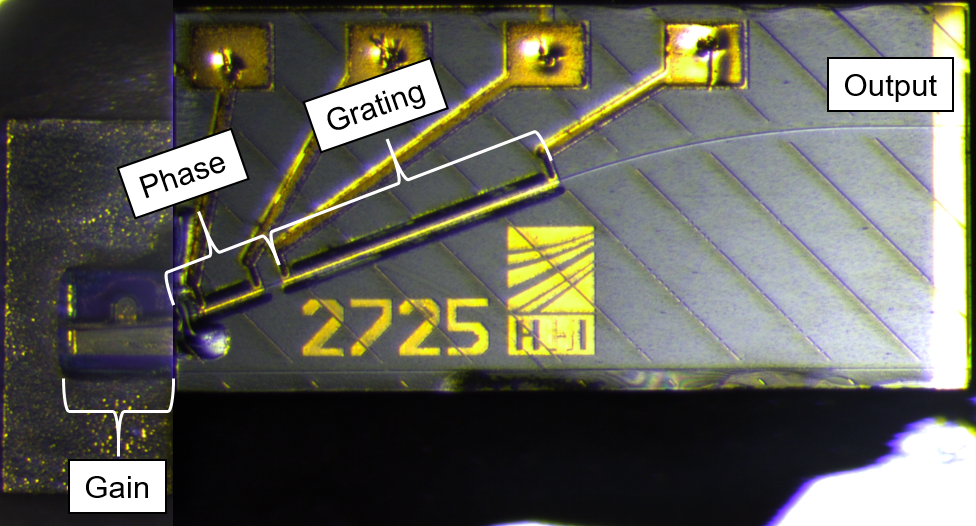
\includegraphics[width=.9\linewidth]{figures/tunable_DBR.png}
    \caption{Illustration of a tubale three-section DBR laser constructed by combining polymer-based phase and grating section with an active Indium Phosphide (InP) based gain section. The cleaved facet at the output waveguide side may introduce feedback effects depending on the way it is characterized.}
    \label{fig:tunable_DBR}
\end{figure}